\documentclass{article}
\usepackage{graphicx} % Required for inserting images
\usepackage[backend=biber]{biblatex}
\addbibresource{bibliography.bib}

\title{Machine Learning For Data Science I, \\[0.1cm] Homework 01}

\author{Maj Gaberšček, 27212075}
\date{March 2023}

\begin{document}

\maketitle

\section{Problem}

This homework's task was implementation of decision trees and random forests in the programming language \texttt{Python}.

Decision tree and Random forest needed to be implemented as classes. Classes were supposed to have methods for building decision trees or random forests on numerical data with binary target variables. They were also supposed to contain methods, that provide predicting with already trained decision tree or random forest. Random forest should also have a method importance, which calculates each attribute's importance, as described in \cite{rand_for}.

\section{Implementation}

\subsection{Overview}

All code is provided in file \texttt{hw\_tree.py}. Decision trees and Random forests are provided as classes with different methods. There are also some auxiliary functions, that solve different subproblems. Each function is well documented. In the end, we import the \emph{Fourier-transform infrared spectroscopy} dataset and apply it to Decision trees and Random forests. 

\subsection{Decision tree}

Decision tree skeleton is implemented as a class, \texttt{Tree}. We can initialize it, by specifying different parameters, such as random generator or minimal number of samples (to continue with tree expansion). \texttt{Tree} also consists of method \texttt{build}, which fits a tree to training array of attribute values, \texttt{X} and target array \texttt{y}. This method then returns an object of type \texttt{TreeNode}, which represents a node in a tree (either a decision node or a leaf node). Tree is being fitted by an auxiliarry function \texttt{recursively\_build}.

The \texttt{TreeNode} class represents a node of a tree. The node can be of two types: a decision node or a leaf (also called terminal nodes). A \textbf{decision node} breaches the tree into two subtrees, left subtree and right subtree, which are also of type \texttt{TreeNode}. It also has two other attributes: \texttt{attribute}, which tells us, by which attribute we are splitting the tree and \texttt{value}, which is a value, by which we split. For example, if we are splitting by attribute 10 and value 25, left subtree in fitted on subdata, which has attribute 10 less or equal to 25, and the right subtree is fitted on subdata, which has attribute 10 greater then 25. If \texttt{TreeNode} represents a leaf of a tree, it only has one attribute, which is the prediction class (0 or 1 in our case). \texttt{TreeNode} also has a method \texttt{predict}, which is also recursivelly written. It checks if \texttt{TreeNode} is a decision node or a leaf. If it is a leaf it returns prediction. If it is a decision node, it checks the input attributes (values, which we want to predict the target on) and predicts on suitable subtree (depends on value and attribute of the tree).

\subsection{Random forest}

The skeleton for Random forests is in class \texttt{RandomForest}. This class contains a tree skeleton as an attribute, along with attributes for number of trees in the random forest and random generator attribute. It also has a \texttt{build} method, which fits a tree on data and creates a \texttt{RFModel} object, which represents a model forest, fitted on \texttt{X} and \texttt{y}.

\texttt{RFModel} represents a trained model and it has the following attributes: \texttt{trees}, which is a list of trees in the forest; \texttt{X}, \texttt{y} and \texttt{rand}, a random generator. There is a method \texttt{predict}, which iterates over a trees and predict the target in each tree. Then each tree votes, and the class with majority of votes is returned by the random tree. Second method in random forest model is \texttt{importance}. It calculates importance of each attribute of the dataset \texttt{X} and then returns array with importances.

\section{Results}

First we built a full decision tree (minimum samples to still continue breaching is 2) on the \emph{Fourier-transform infrared spectroscopy} dataset. Firstly we test our model on training data. As expected, model returned a 100\% accuracy (misclassification rate was 0, as well as the standard error). Then we tested our model on testing dataset (which was not used when fitting the tree). We got missclassification rate of 25,8\% and standard error 0,06.

Random forest was built and fitted on the same dataset (\emph{Fourier-transform infrared spectroscopy}). Forest consisted of 100 trees, which used random square root number of attributes for breaching. Again, as already expected: when testing on training data, we got misclassification rate and standard error 0. When testing on testing data, missclassification rate was 1,72\%, which is a lot better then one full decision tree. Standard error was 0,02.

Lastly, we calculated parameter importance for random forest, built as discussed previously. Then we plotted the returned data, which can be seen in Figure \ref{fig:example}. Higher importance means, that attribute contributes more to the final prediction.

\begin{figure}[ht]
  \centering
  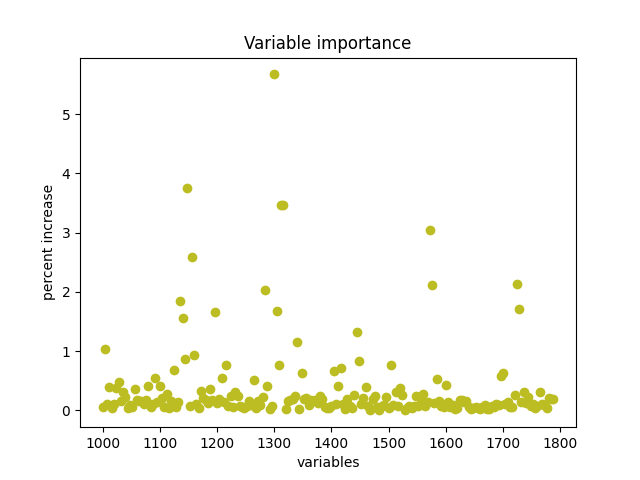
\includegraphics[width=1\textwidth]{importance.png}
  \caption{Importance of attributes in a random tree on Fourier-transform infrared spectroscopy data}
  \label{fig:example}
\end{figure}


\printbibliography

\end{document}